\chapter{Propuesta}

\section{Descripcion detallada}

La app presentada daría la mayoría de funcionalidades de pago de una manera gratuita y aporta su funcionalidad de medir de forma personalizada el rendimiento del deportista. También se añade una IA, una funcionalidad que no vista en muchas aplicaciones del sector y si existen, son de pago. La función de la inteligencia artificial sería la de aconsejar al usuario cuando este lo necesite, sobre su rendimiento y/o parámetros medidos durante su entrenamiento.
Para clarificar las diferencias con el resto de apps del mercado:

\begin{landscape}
\begin{figure}[H]
   \centering
    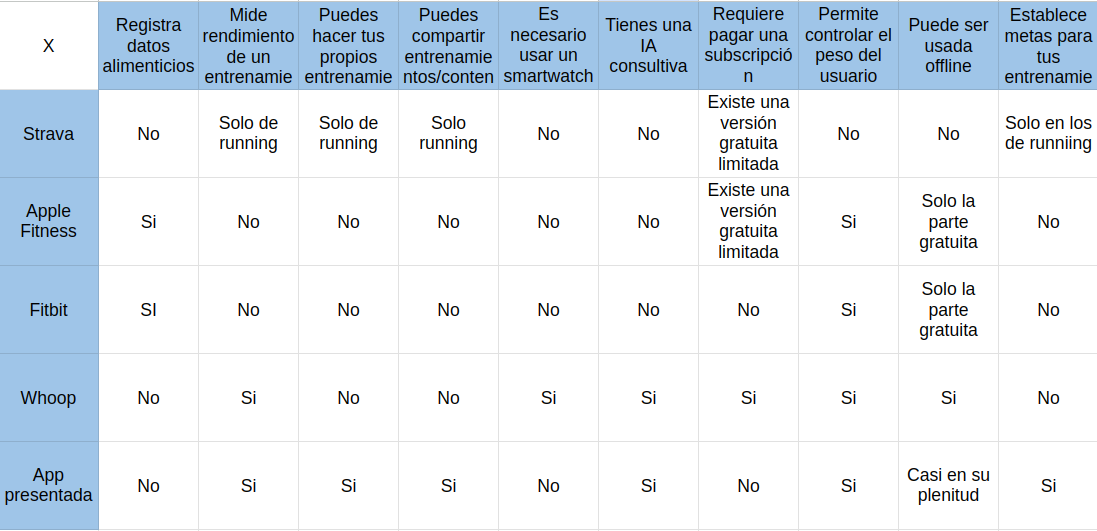
\includegraphics[width=1.65\textwidth]{tablas/tabla.png}
    \caption{Tabla comparativa}
    \label{fig:Tabla comparativa}
\end{figure} 
\end{landscape}

\section{Elección de tecnologías}

\section{Backend}

Se usará Express.js(Node.js), la principal razón que se tiene para optar por esta tecnología, es la gran familiaridad que se tiene con el entorno de JavaScript, se conocen las tecnologías y la forma de implementación, su gran flexibilidad para implementar muchas funcionalidades diversas también fué una buena baza para escoger esta herramienta.
Django fué la primera descartada, porque como bien dice en la tabla de la sección anterior(\cref{fig:Tabla backend}) está más enfocado a proyectos de gran envergadura.
Ruby on Rails fue la que más dudas planteó, como se dijo anteriormente es muy buena opción para las metodologías ágiles y como se dirá más adelante, se optará por una metodología ágil para el desarrollo. Pero al final se descartó por el desconocimiento de la herramienta.

\section{Frontend}

Se ha decidido usar Flutter, dado que Xamarin es buena herramienta, pero está más enfocada a un desarrollo en un ambiente Microsoft.
React Native también es una buena herramienta, fue principalmente la que más dudas sembró, ya que como se dijo previamente se usará un backend basado en Express.js, esto entonces permitiría unificar entornos lo cual favorecería al desarrollo. pero se descartó por lo personalizable que son las IUs desarrolladas en Flutter respecto a esta tecnología.

\section{Base de datos}

Para las bases de datos, tanto para el backend como para la local de la app se usará una SQL, dado a la familiaridad que se dispone con esta tecnología y la necesidad de unificar el tipo de tecnología del servidor y de la app. Esto anterior se debe a que como bien se ha dicho se usará Flutter como entorno frontend y la herramienta que se facilita para el almacenamiento local en este es SQlite, basada en un modelo relacional.

Los modelos NoSQL, se descartaron principalmente porque las relaciones entre elementos suelen ser más complejas y en este proyecto pueden enrevesarse facilmente.

\section{Diagrama de arquitectura}

\begin{figure}[H]
   \centering
    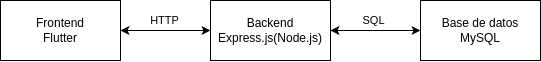
\includegraphics[width=\textwidth]{tablas/Arq.png}
    \caption{Tabla comparativa}
    \label{fig:Tabla comparativa}
\end{figure} 

\section{Metodología utilizada}
Para el desarrollo de esta app, se usará una metodología \textit{ágil} tipo \textbf{SCRUM}. Se decidió usar esta porque permite corregir fallos en la velocidad de diseño y/o planificación de forma eficiente y sin dañar el producto final. Esta metodología permite también entregar desarrollos funcionales a la tutora e ir validando las funcionalidades poco a poco mediante reuniones.

Las reuniones con la tutora serán las \textit{sprint reviews}.

\section{Temporización}
La temporización se realizó el día 25 de marzo de 2025. La entrega del producto (este TFG) está prevista para el 16 de junio de 2025, es decir, 83 días, o lo que es lo mismo, casi 12 semanas. Si un sprint dura 2 semanas, habrá 6 sprints hasta la entrega final.

La iteración 0 se dedicará al diseño de pantallas y al repaso de las funcionalidades de la app, para concretar las historias de usuario y sus prioridades. La idea inicial es dividir la app en varios módulos y centrar cada sprint en cada uno de ellos:

\begin{enumerate}
  \item Diagramas de la app y ejercicios
  \item Rutinas, usuarios y sesión
  \item Datos que ingresa el usuario
  \item Flujo de entrenamiento
  \item Inteligencia Artificial (IA)
  \item Smartwatch
\end{enumerate}

\section{Seguimiento del desarrollo}

\subsection{Iteración 0}
En esta primera iteración me centré en realizar los diseños de la app, considerando su accesibilidad. También concreté el \textit{product backlog}, compuesto por 41 historias de usuario. En las historias no menciono ningún actor puesto que solo existe el usuario que realiza los ejercicios y el es protagonista en todas ellas, no hay ningún moderador.

A pesar de trabajar con SCRUM se realizarán todos los diseños de interfaces de usuario en este primer sprint para concretar con la tutora los requisitos principales de la aplicación a desarrollar en este TFG. En nuestro caso los diseños de las interfaces se usarán como herramientas de captura y especificación de requisitos. En cada iteración se podrán revisar si hay cambios. 


La lista inicial de historias de usuario es la siguiente, y algunas incluyen tareas secundarias:

\begin{description}
  \item[\textbf{SCRUM-1}] Registrar peso por día
  \item[\textbf{SCRUM-2}] Establecer peso objetivo
  \item[\textbf{SCRUM-3}] Insertar/Borrar/Modificar ejercicio de la lista de ejercicios
  \item[\textbf{SCRUM-4}] Buscar rutina en la lista del usuario
  \item[\textbf{SCRUM-5}] Sustituir un ejercicio por otro en la rutina
  \item[\textbf{SCRUM-6}] Insertar/Borrar/Modificar rutina
  \item[\textbf{SCRUM-7}] Poner una meta en cada ejercicio
  \item[\textbf{SCRUM-8}] Hacer grafica de los datos de los ejercicios
  \item[\textbf{SCRUM-9}] Revisar datos para ver si el descanso es necesario
  \item[\textbf{SCRUM-10}] Enseñar datos de una rutina a descargar
  \item[\textbf{SCRUM-11}] Compartir mi rutina
  \item[\textbf{SCRUM-12}] Guardar las repeticiones y series de todos los ejercicios de un entrenamiento
  \item[\textbf{SCRUM-13}] Valorar el entrenamiento en base a la marca actual y la meta del usuario
  \item[\textbf{SCRUM-14}] Monitorizar pulso en tiempo real
  \item[\textbf{SCRUM-15}] Medir pulso en reposo y compararlo con datos de ejercicios
  \item[\textbf{SCRUM-16}] Avisar de anomalías en el pulso de forma suave
  \item[\textbf{SCRUM-17}] Obtener calorías quemadas
  \item[\textbf{SCRUM-18}] Comprobar el equilibrio nervioso del usuario
  \item[\textbf{SCRUM-19}] Realizar el flujo del entrenamiento
  \item[\textbf{SCRUM-20}] Conectar con la IA para iniciar diálogo
  \item[\textbf{SCRUM-21}] Crear/Borrar usuario
  \item[\textbf{SCRUM-22}] Resumir datos
  \item[\textbf{SCRUM-23}] Iniciar/Cerrar sesión
  \item[\textbf{SCRUM-24}] Medir SpO2
  \item[\textbf{SCRUM-25}] Interpretar constantes
  \item[\textbf{SCRUM-26}] Buscar ejercicios en la lista de ejercicios
  \item[\textbf{SCRUM-27}] Hacer la IU de la lista de los ejercicios
  \item[\textbf{SCRUM-28}] Hacer la IU de creación de ejercicio
  \item[\textbf{SCRUM-29}] Pop up de confirmación
  \item[\textbf{SCRUM-30}] Hacer IU de datos ejercicio
  \item[\textbf{SCRUM-31}] Crear IU de la lista de las rutinas
  \item[\textbf{SCRUM-32}] Crear IU de pantalla inicial
  \item[\textbf{SCRUM-33}] Crear IU menú principal
  \item[\textbf{SCRUM-34}] Crear IU datos rutinas
  \item[\textbf{SCRUM-35}] IU lista ejercicios de rutina modificable
  \item[\textbf{SCRUM-36}] Crear IU para crear rutina
  \item[\textbf{SCRUM-36}] Detectar metas cumplidas despues del entrenamiento
  \item[\textbf{SCRUM-37}] Crear IU del perfil del usuario
  \item[\textbf{SCRUM-38}] Detectar metas cumplidas en los ejercicios despues del entrenamiento
  \item[\textbf{SCRUM-39}] Buscar rutinas para descargar
  \item[\textbf{SCRUM-40}] IU del pop up de resumir datos
  \item[\textbf{SCRUM-41}] IU desplegable rutina
  
\end{description}

A continuación se muestran los diseños creados en esta iteración:

\textbf{Inicio de sesion y crear usuario}

\begin{figure}[H]
   \centering
    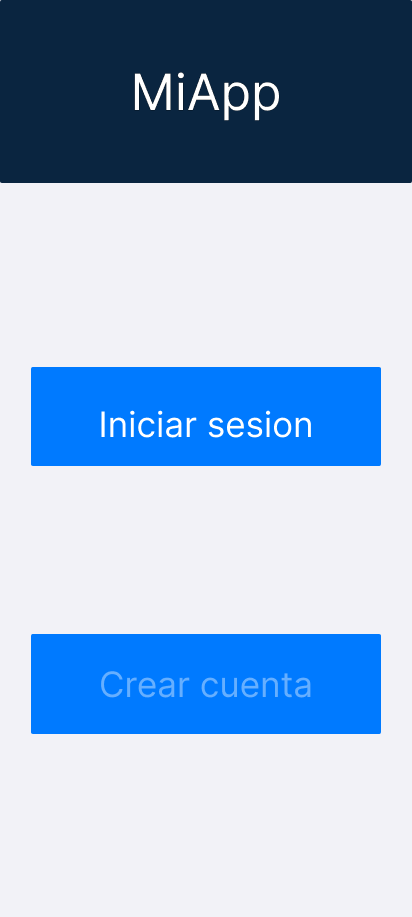
\includegraphics[width=0.6\textwidth]{fotos/Frame 22.png}
    \caption{Pagina inicial}
    \label{fig:Pagina inicial}
\end{figure}
\begin{figure}[H]
   \centering
    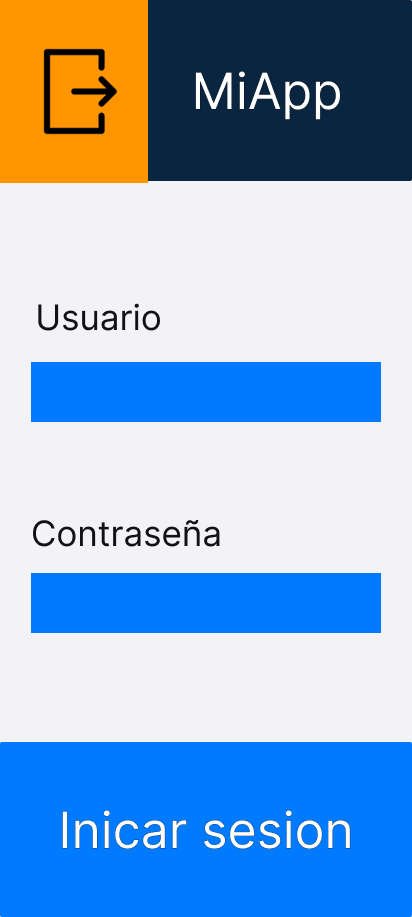
\includegraphics[width=0.6\textwidth]{fotos/Frame 22-1.png}
    \caption{Inicio de sesion}
    \label{fig:Inicio de sesion}
\end{figure}
\begin{figure}[H]
   \centering
    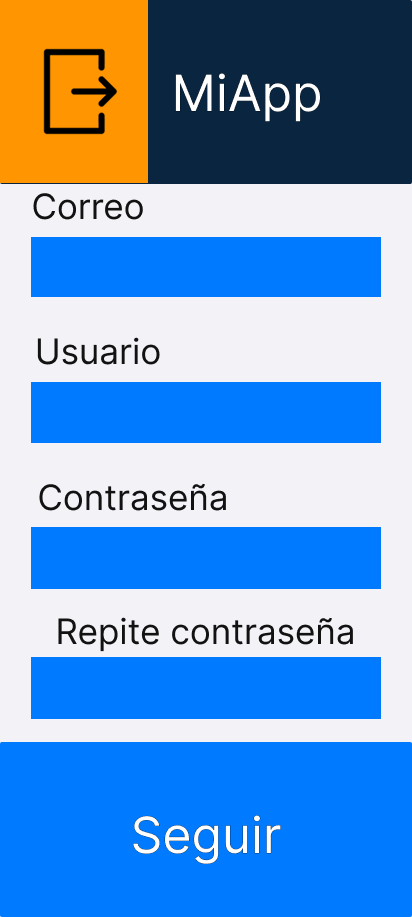
\includegraphics[width=0.6\textwidth]{fotos/Frame 24.png}
    \caption{Crear cuenta 1}
    \label{fig:Crear cuenta 1}
\end{figure}
\begin{figure}[H]
   \centering
    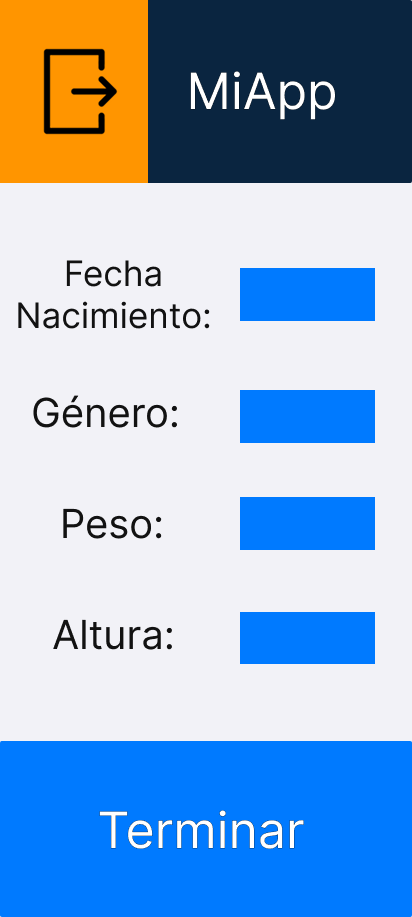
\includegraphics[width=0.6\textwidth]{fotos/Frame 25.png}
    \caption{Crear cuenta 2}
    \label{fig:Crear cuenta 2}
\end{figure}

\textbf{Menu principal}

\begin{figure}[H]
   \centering
    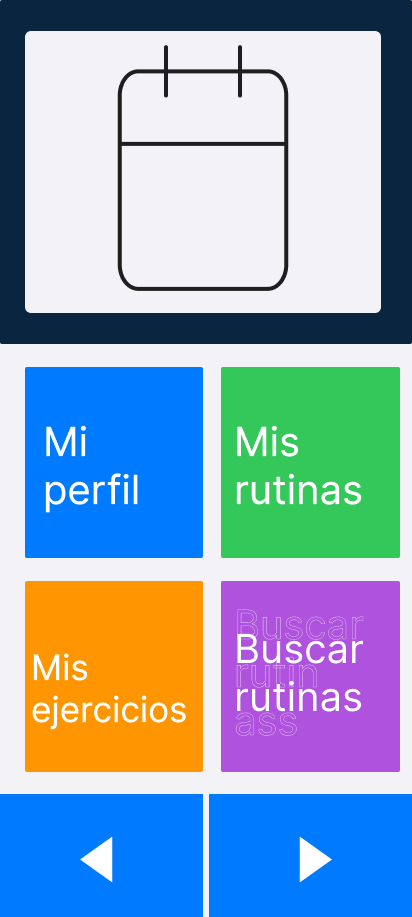
\includegraphics[width=0.6\textwidth]{fotos/Frame 30.png}
    \caption{Menu principal}
    \label{fig:Menu principal}
\end{figure}

\textbf{Lista ejercicios del usuario}

\begin{figure}[H]
   \centering
    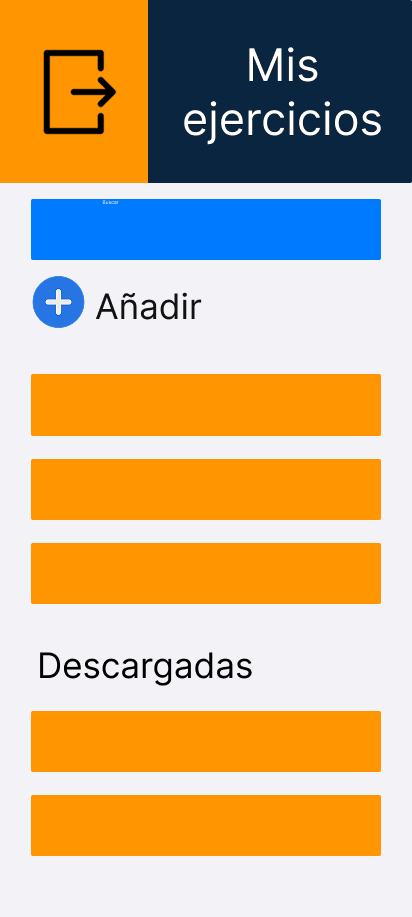
\includegraphics[width=0.6\textwidth]{fotos/Frame 40.png}
    \caption{Lista ejercicios}
    \label{fig:Lista ejercicios}
\end{figure}
\begin{figure}[H]
   \centering
    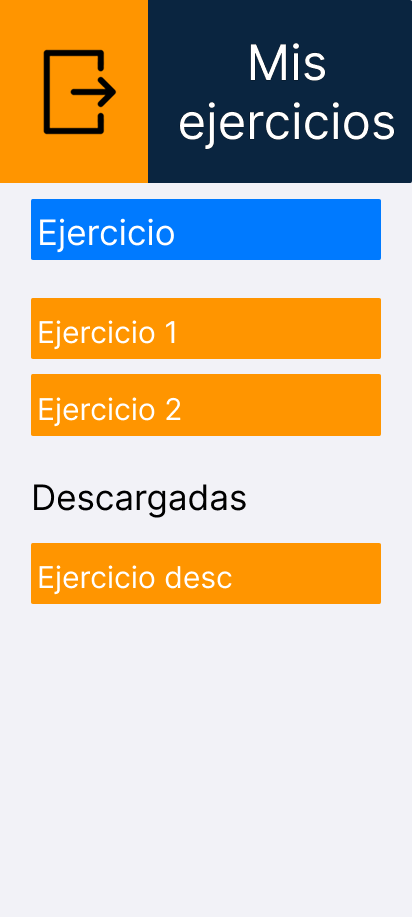
\includegraphics[width=0.6\textwidth]{fotos/Frame 41.png}
    \caption{Lista ejercicios filtrada}
    \label{fig:Lista ejercicios filtrada}
\end{figure}
\begin{figure}[H]
   \centering
    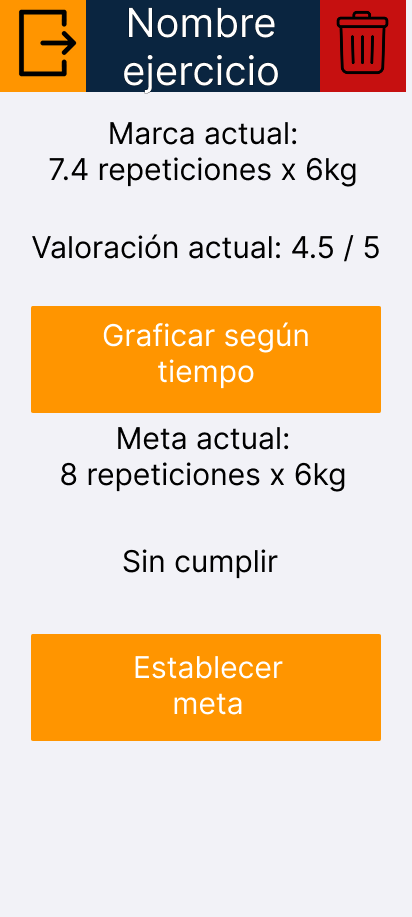
\includegraphics[width=0.6\textwidth]{fotos/Frame 42.png}
    \caption{Datos ejercicio}
    \label{fig:Datos ejercicio}
\end{figure}
\begin{figure}[H]
   \centering
    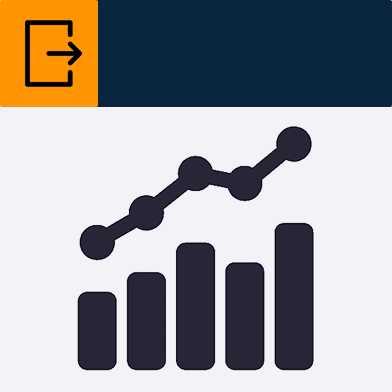
\includegraphics[width=0.6\textwidth]{fotos/Frame 43.png}
    \caption{Pop up graficar segun tiempo}
    \label{fig:Pop up graficar segun tiempo}
\end{figure}
\begin{figure}[H]
   \centering
    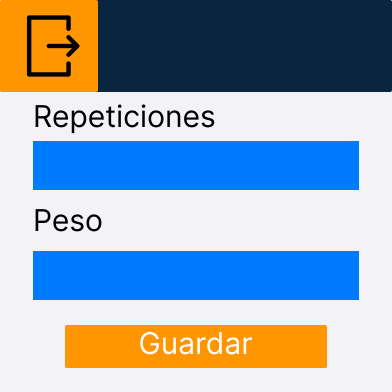
\includegraphics[width=0.6\textwidth]{fotos/Frame 45.png}
    \caption{Pop up establecer meta}
    \label{fig:Pop up establecer meta}
\end{figure}
\begin{figure}[H]
   \centering
    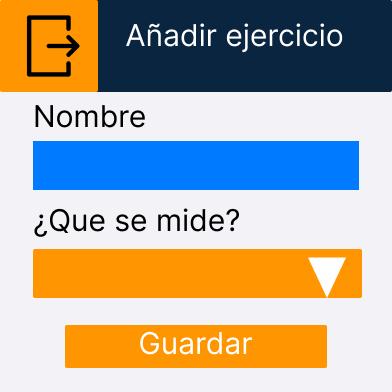
\includegraphics[width=0.6\textwidth]{fotos/Frame 64.png}
    \caption{Pop up crear ejercicio}
    \label{fig:Pop up crear ejercicio}
\end{figure}

\textbf{Lista rutinas}

\begin{figure}[H]
   \centering
    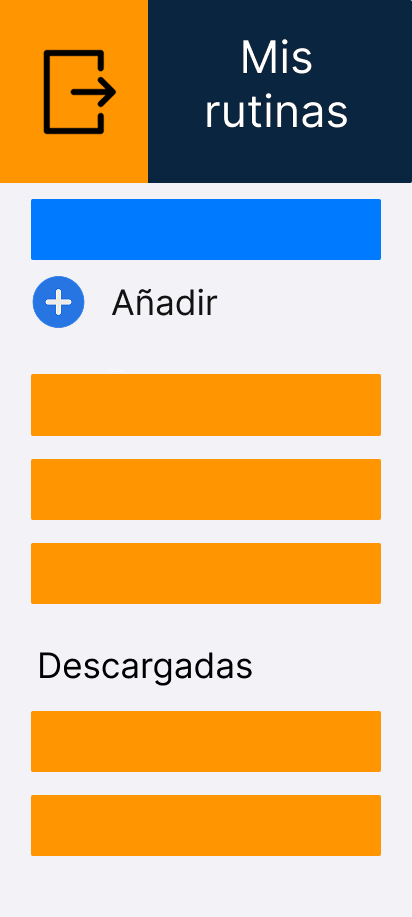
\includegraphics[width=0.6\textwidth]{fotos/Frame 46.png}
    \caption{Lista rutinas}
    \label{fig:Lista rutinas}
\end{figure}
\begin{figure}[H]
   \centering
    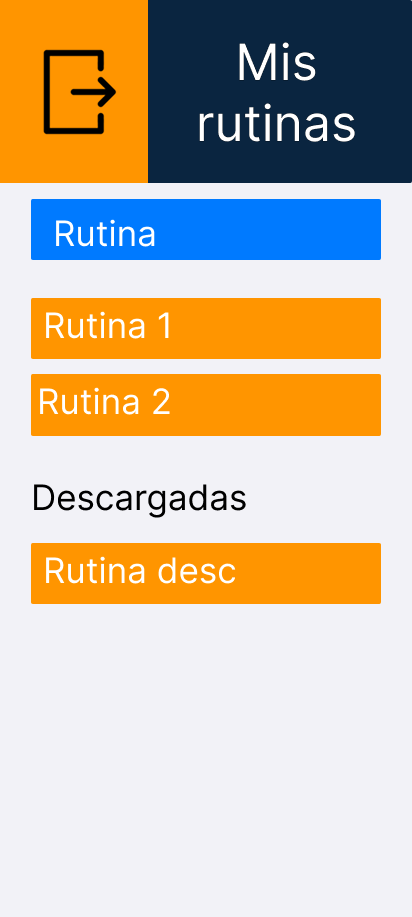
\includegraphics[width=0.6\textwidth]{fotos/Frame 47.png}
    \caption{Lista rutinas filtradas}
    \label{fig:Lista rutinas filtradas}
\end{figure}
\begin{figure}[H]
   \centering
    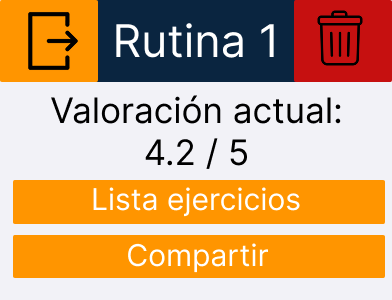
\includegraphics[width=0.6\textwidth]{fotos/Frame 48.png}
    \caption{Datos rutina modificable}
    \label{fig:Datos rutina modificable}
\end{figure}
\begin{figure}[H]
   \centering
    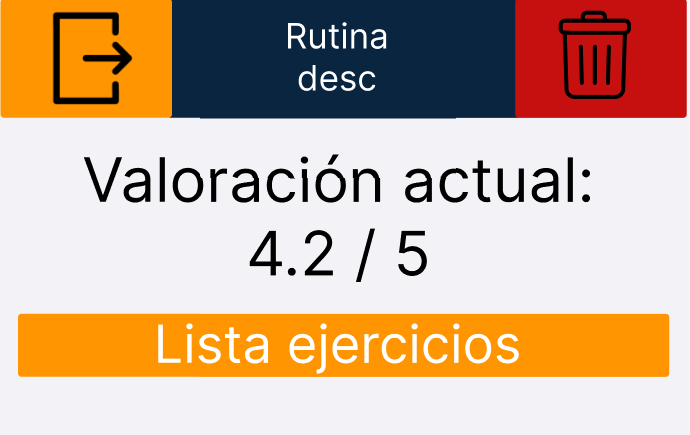
\includegraphics[width=0.6\textwidth]{fotos/Frame 49.png}
    \caption{Datos rutina no modificable}
    \label{fig:Datos rutina no modificable}
\end{figure}
\begin{figure}[H]
   \centering
    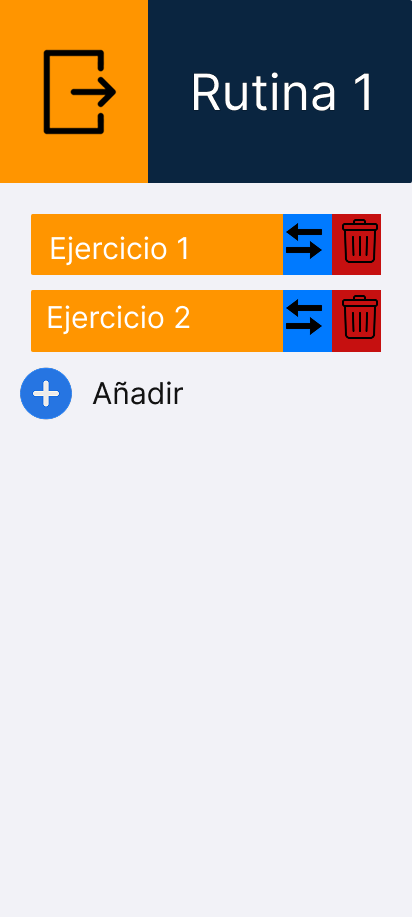
\includegraphics[width=0.6\textwidth]{fotos/Frame 50.png}
    \caption{Modificar ejericios rutina}
    \label{fig:Modificar ejericios rutina}
\end{figure}
\begin{figure}[H]
   \centering
    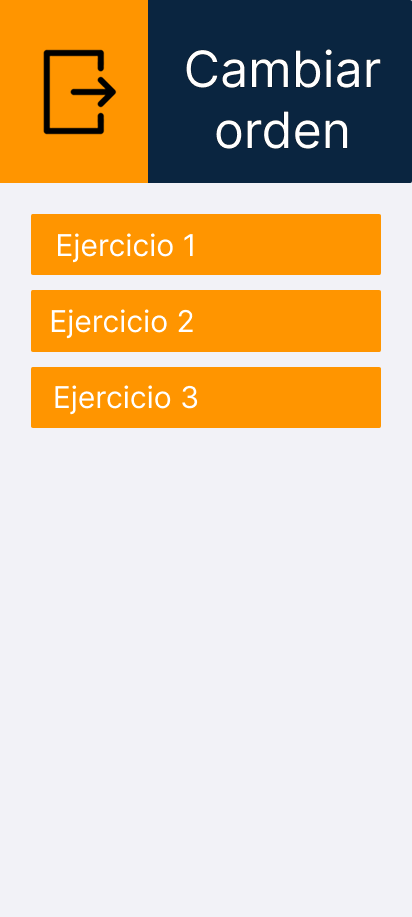
\includegraphics[width=0.6\textwidth]{fotos/Frame 51.png}
    \caption{Cambiar orden ejercicios rutina}
    \label{fig:Cambiar orden ejercicios rutina}
\end{figure}
\begin{figure}[H]
   \centering
    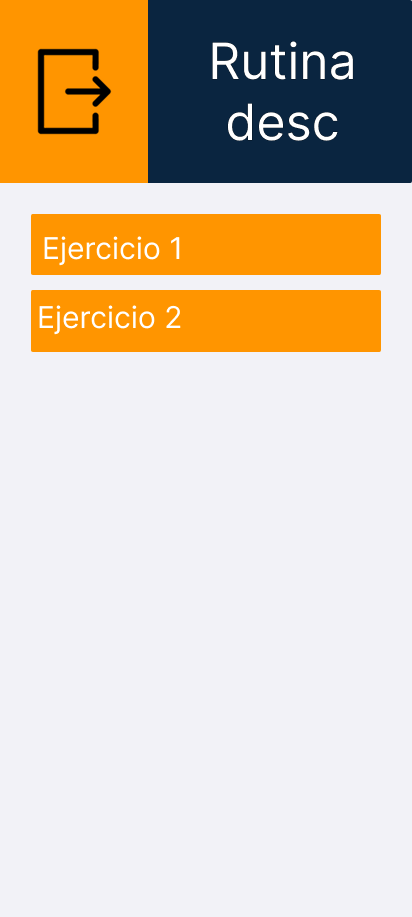
\includegraphics[width=0.6\textwidth]{fotos/Frame 52.png}
    \caption{Ejercicios rutina descargada}
    \label{fig:Ejercicios rutina descargada}
\end{figure}
\begin{figure}[H]
   \centering
    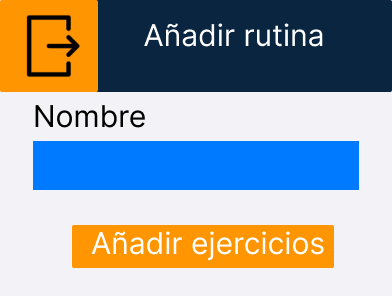
\includegraphics[width=0.6\textwidth]{fotos/Frame 65.png}
    \caption{Pop up crear rutinas}
    \label{fig:Pop up crear rutinas}
\end{figure}

\textbf{Mi perfil}

\begin{figure}[H]
   \centering
    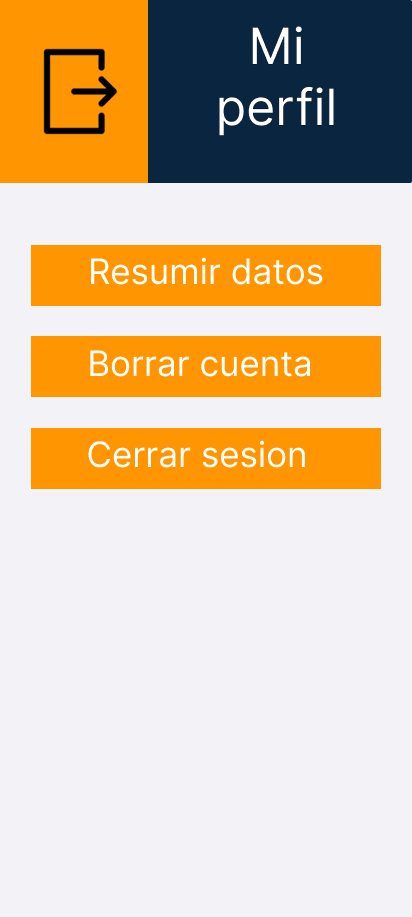
\includegraphics[width=0.6\textwidth]{fotos/Frame 36.png}
    \caption{Opciones de perfil usuario}
    \label{fig:Opciones de perfil usuario}
\end{figure}
\begin{figure}[H]
   \centering
    
\includegraphics[width=0.75\textwidth]{fotos/Frame 38.png}
    \caption{Pop up de confirmacion}
    \label{fig:Pop up de confirmacion}
\end{figure}
\begin{figure}[H]
   \centering
    
\includegraphics[width=0.75\textwidth]{fotos/Frame 39.png}
    \caption{Pop up de confirmacion resumir datos}
    \label{fig:Pop up de confirmacion resumir datos}
\end{figure}

\textbf{Buscar rutina para descargar}

\begin{figure}[H]
   \centering
    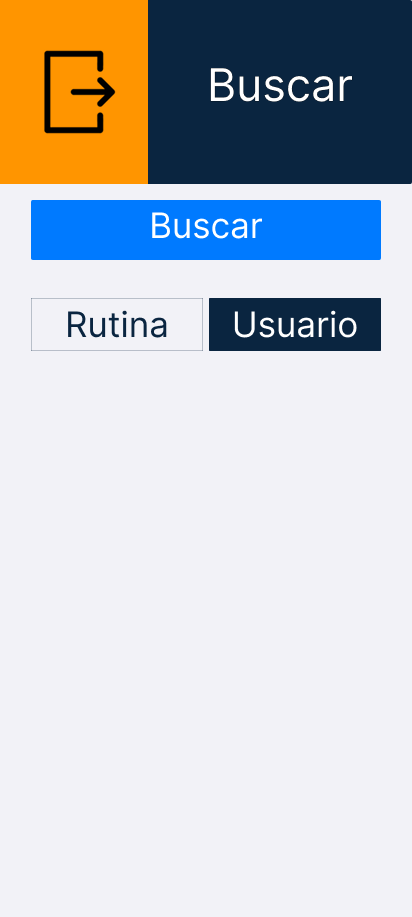
\includegraphics[width=0.6\textwidth]{fotos/Frame 53.png}
    \caption{Buscar usuario}
    \label{fig:Buscar usuario}
\end{figure}
\begin{figure}[H]
   \centering
    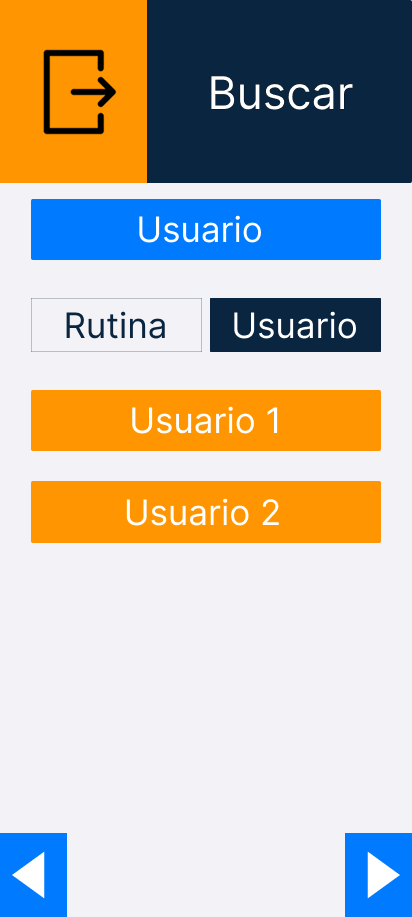
\includegraphics[width=0.6\textwidth]{fotos/Frame 54.png}
    \caption{Buscar usuario filtrado}
    \label{fig:Buscar usuario filtrado}
\end{figure}
\begin{figure}[H]
   \centering
    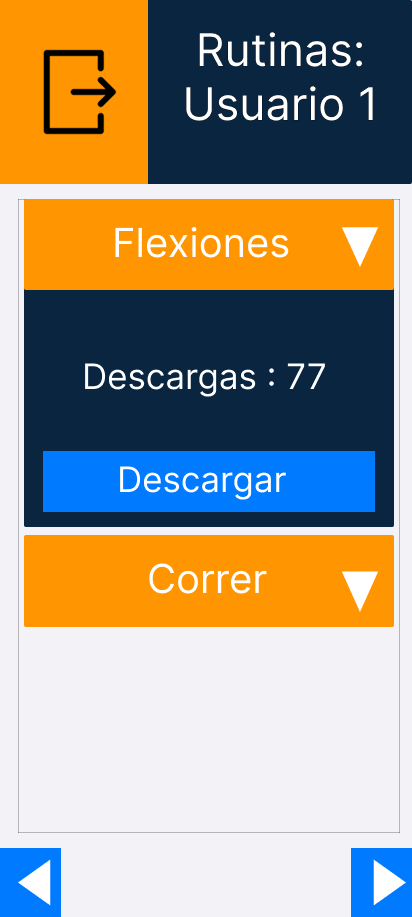
\includegraphics[width=0.6\textwidth]{fotos/Frame 56.png}
    \caption{Rutinas de un usuario}
    \label{fig:Rutinas de un usuario}
\end{figure}
\begin{figure}[H]
   \centering
    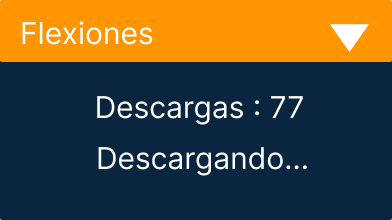
\includegraphics[width=0.6\textwidth]{fotos/Frame 57.png}
    \caption{Widget descargar rutina}
    \label{fig:Widget descargar rutina}
\end{figure}
\begin{figure}[H]
   \centering
    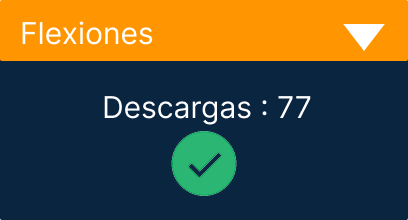
\includegraphics[width=0.6\textwidth]{fotos/Frame 58.png}
    \caption{Widget rutina descargada}
    \label{fig:Widget rutina descargada}
\end{figure}
\begin{figure}[H]
   \centering
    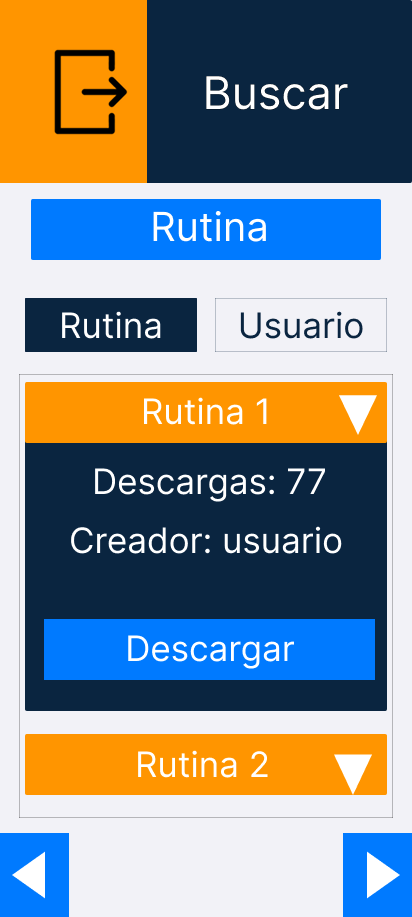
\includegraphics[width=0.6\textwidth]{fotos/Frame 59.png}
    \caption{Buscar rutinas por su nombre filtrada}
    \label{fig:Buscar rutinas por su nombre filtrada}
\end{figure}

\textbf{Entrenamiento (Una vez seleccionada una fecha en el calendario del menu principal saldría la siguiente ventana)}

\begin{figure}[H]
   \centering
    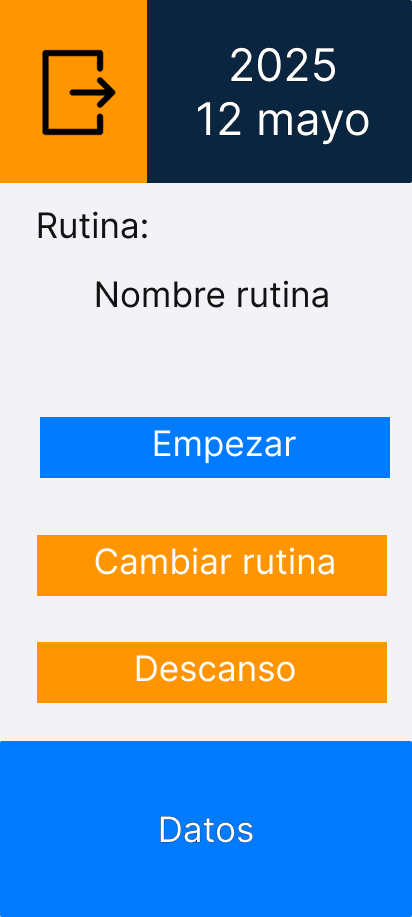
\includegraphics[width=0.6\textwidth]{fotos/Frame 26.png}
    \caption{Entrenamiento de un día determinado}
    \label{fig:Entrenamiento de un día determinado}
\end{figure}
\begin{figure}[H]
   \centering
    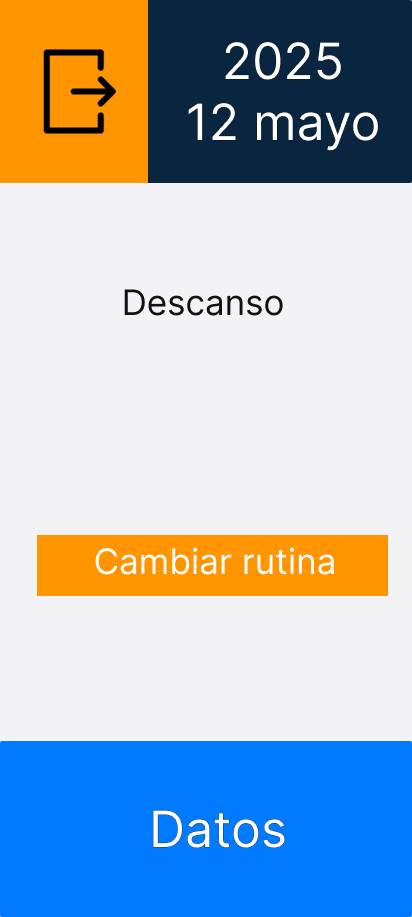
\includegraphics[width=0.6\textwidth]{fotos/Frame 27.png}
    \caption{Descanso en un día determinado}
    \label{fig:Descanso en un día determinado}
\end{figure}

Si seleccionamos datos de una fecha saldría esto
\begin{figure}[H]
   \centering
    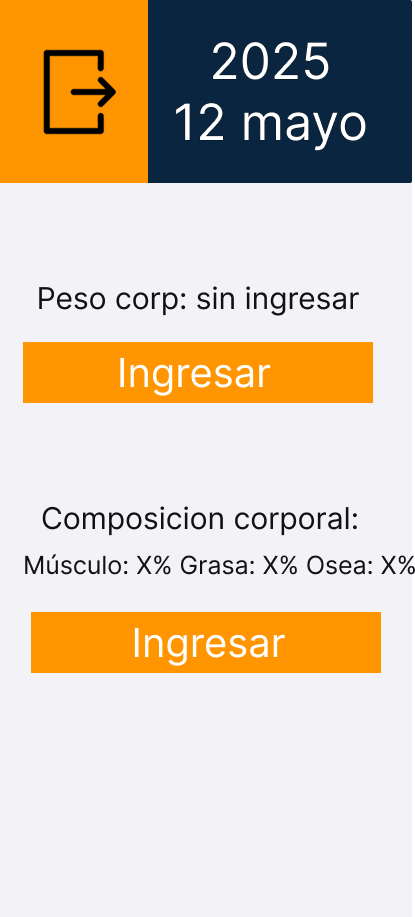
\includegraphics[width=0.6\textwidth]{fotos/Frame 29.png}
    \caption{Frame 29.png}
    \label{fig:Frame_29}
\end{figure}

La siguiente pantalla sale al comenzar el entrenamiento
\begin{figure}[H]
   \centering
    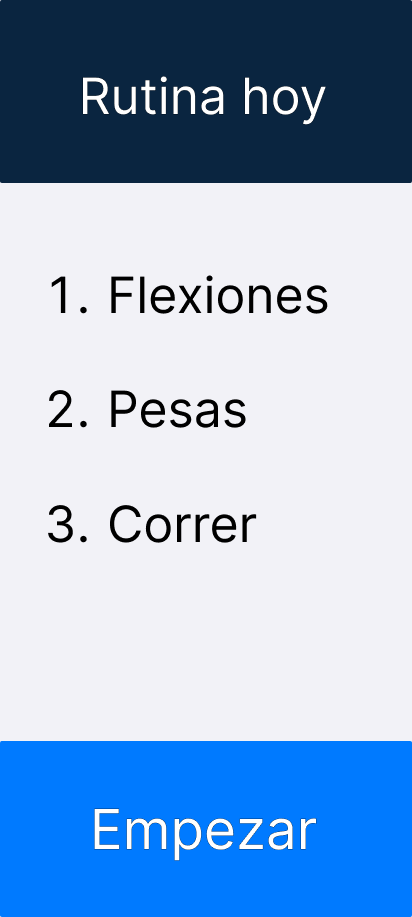
\includegraphics[width=0.6\textwidth]{fotos/Frame 1.png}
    \caption{Lista ejercicios del entrenamiento actual}
    \label{fig:Lista ejercicios del entrenamiento actual}
\end{figure}
\begin{figure}[H]
   \centering
    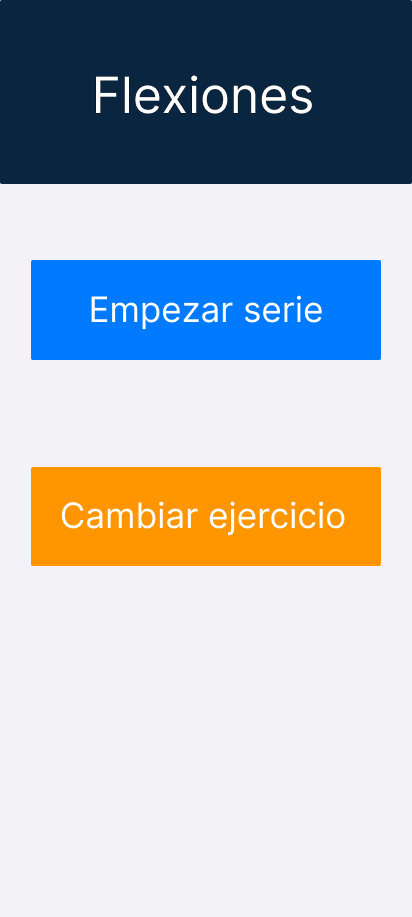
\includegraphics[width=0.6\textwidth]{fotos/Frame 2.png}
    \caption{Primera serie flexiones}
    \label{fig:Primera serie flexiones}
\end{figure}
\begin{figure}[H]
   \centering
    
\includegraphics[width=0.6\textwidth]{fotos/Frame 3.png}
    \caption{Realizando flexiones}
    \label{fig:Realizando flexiones}
\end{figure}
\begin{figure}[H]
   \centering
    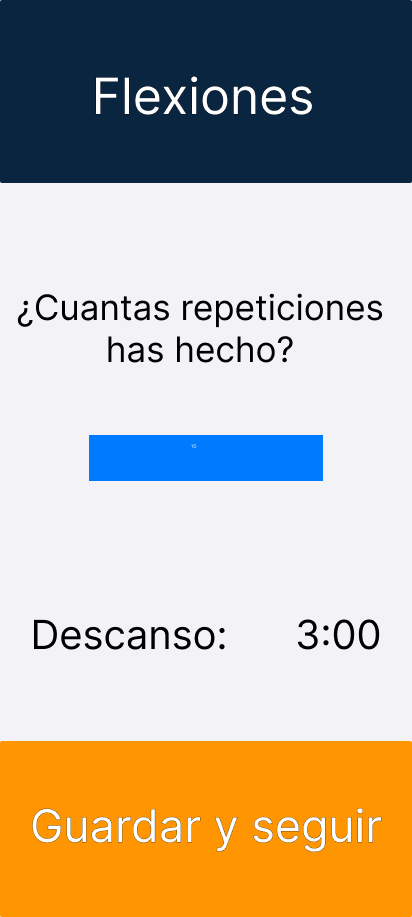
\includegraphics[width=0.6\textwidth]{fotos/Frame 4.png}
    \caption{Fin de la serie(Descanso no completado)}
    \label{fig:Fin de la serie(Descanso no completado)}
\end{figure}
\begin{figure}[H]
   \centering
    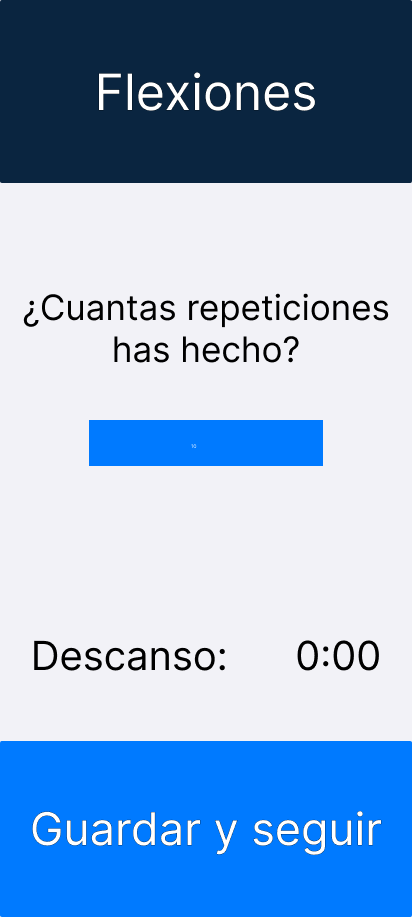
\includegraphics[width=0.6\textwidth]{fotos/Frame 5.png}
    \caption{Fin de la serie(Descanso completado)}
    \label{fig:Fin de la serie(Descanso completado)}
\end{figure}
\begin{figure}[H]
   \centering
    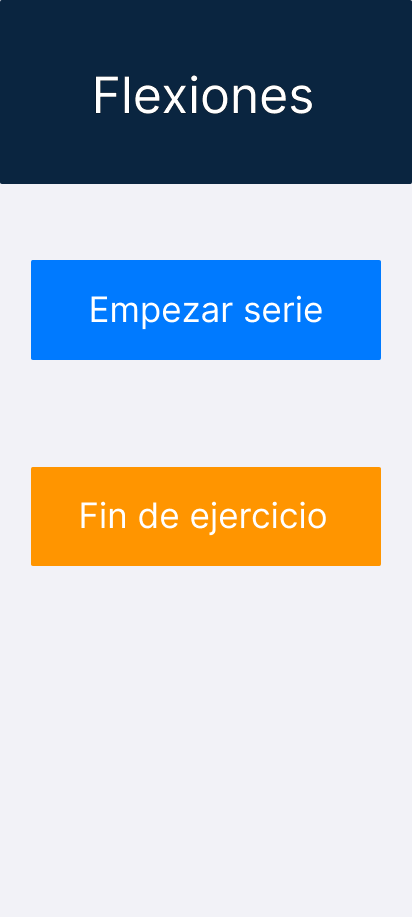
\includegraphics[width=0.6\textwidth]{fotos/Frame 62.png}
    \caption{Acabar ejercicio o añadir serie}
    \label{fig:Acabar ejercicio o añadir serie}
\end{figure}
\begin{figure}[H]
   \centering
    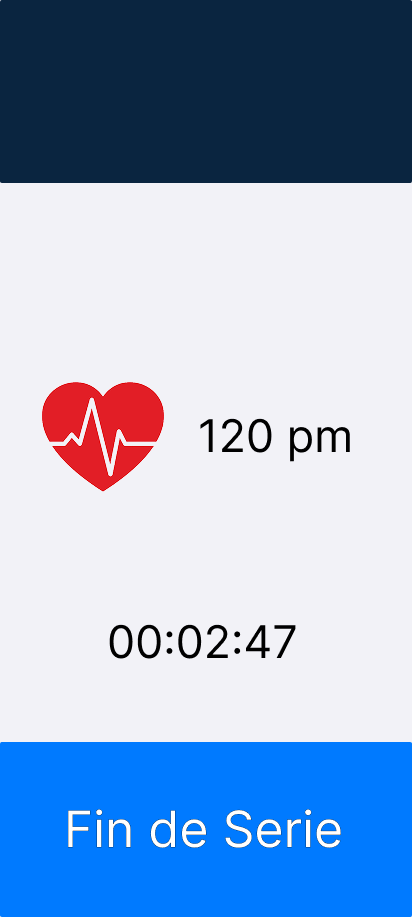
\includegraphics[width=0.6\textwidth]{fotos/Frame 60.png}
    \caption{Realizando ejercicio midiendo tiempo}
    \label{fig:Realizando ejercicio midiendo tiempo}
\end{figure}
\begin{figure}[H]
   \centering
    
\includegraphics[width=0.6\textwidth]{fotos/Frame 20.png}
    \caption{Fin entrenamiento}
    \label{fig:Fin entrenamiento}
\end{figure}
\begin{figure}[H]
   \centering
    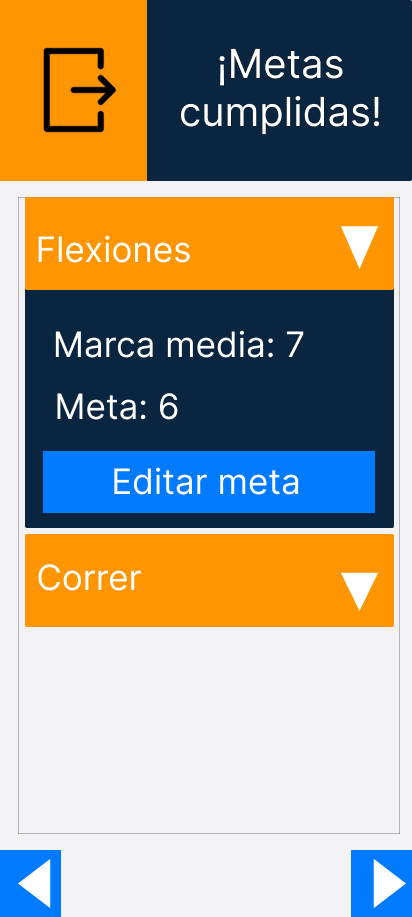
\includegraphics[width=0.6\textwidth]{fotos/Frame 37.png}
    \caption{Metas cumplidas}
    \label{fig:Metas cumplidas}
\end{figure}
\begin{figure}[H]
   \centering
    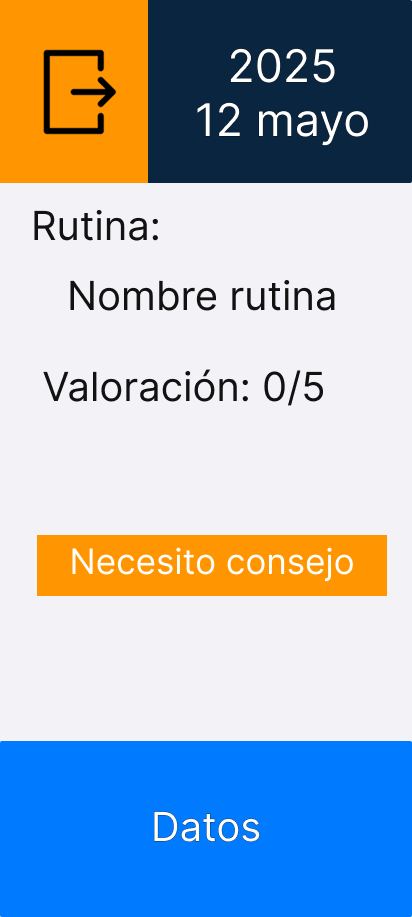
\includegraphics[width=0.6\textwidth]{fotos/Frame 31.png}
    \caption{Datos entrenamiento terminado}
    \label{fig:Datos entrenamiento terminado}
\end{figure}

El chat de la IA se abre cuando se le da a la opcion necesito consejo de un entrenamiento realizado
\begin{figure}[H]
   \centering
    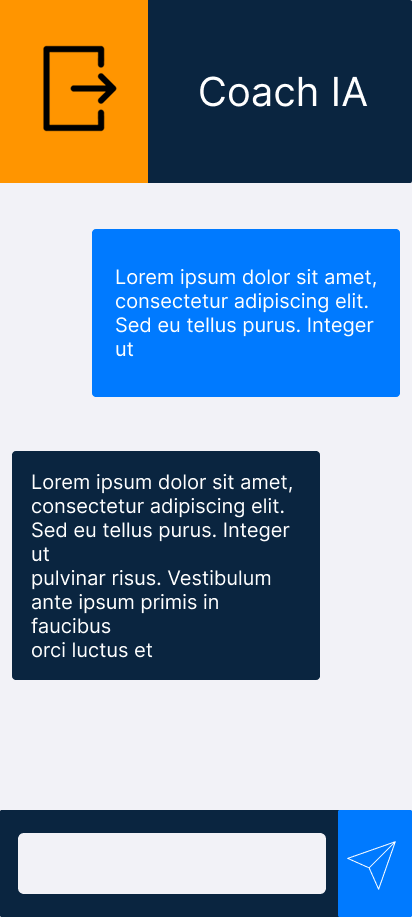
\includegraphics[width=0.6\textwidth]{fotos/Frame 32.png}
    \caption{Chat con IA}
    \label{fig:Chat con IA}
\end{figure}

Si le das a datos de un entrenamiento terminado
\begin{figure}[H]
   \centering
    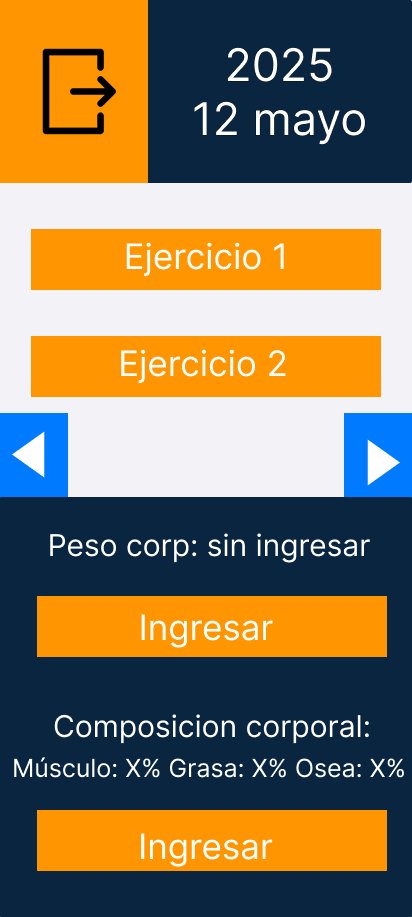
\includegraphics[width=0.6\textwidth]{fotos/Frame 33.png}
    \caption{Datos detallados entrenamiento terminado}
    \label{fig:Datos detallados entrenamiento terminado}
\end{figure}
\begin{figure}[H]
   \centering
    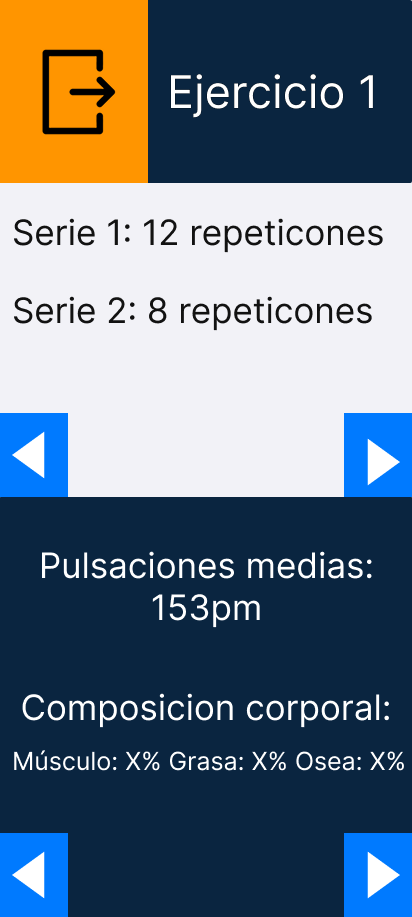
\includegraphics[width=0.6\textwidth]{fotos/Frame 35.png}
    \caption{Pop up datos de un ejercicio en entrenamiento}
    \label{fig:Pop up datos de un ejercicio en entrenamiento}
\end{figure}


Estos diseños pueden cambiar y sufrir alteraciones debido a los sprints reviews y correcciones de accesibilidad. De todas formas, cada cambio será informado con su motivo.

\subsubsection{Sprint Review 0}
Durante esta revisión de sprint se realizaron mejoras de diseño, como la incorporación de iconos en todos los botones para mejorar la accesibilidad. Se revisaron también los títulos de las ventanas, cambiando aquellos que no eran lo suficientemente claros.

Además, se añadieron nuevas historias al \textit{product backlog}, incorporando o desglosando funcionalidades:

\begin{itemize}
  \item SCRUM-42: Copiar rutina
  \item SCRUM-43: Añadir meta por parámetro
  \item SCRUM-44: Solicitar permiso al usuario antes de enviar datos a la IA
  \item SCRUM-45: Enviar datos del entrenamiento actual y anteriores a la IA
  \item SCRUM-46: Conectar/Desconectar con la IA
\end{itemize}

%Muy importante: aquí falta una tabla con todas las historias, priorizadas y organizadas por iteraciones.


\subsection{Iteración 1}
La lista de historias de la primera iteracion queda de la siguiente manera:

\begin{itemize}
    \item SCRUM-26: Buscar ejercicio en lista
    \item SCRUM-3: Insertar/Borrar/Modificar ejercicio de la lista de ejercicios
    \item SCRUM-27: Hacer la IU de la lista de ejercicios ELIMINAR
    \item SCRUM-28: Hacer la IU de creación de ejercicio ELIMINAR
    \item SCRUM-29: Pop up de confirmación
    \item SCRUM-30: Hacer IU de datos ejercicio ELIMINAR
\end{itemize}

A continuación especificaremos las tareas y pruebas de cada historia, y los resultados asociados a cada una. 

\HU{
SCRUM-26: Buscar ejercicio en lista
}{
	\item Implementar la BD local
    \item Implementar algoritmo de búsqueda por nombre
   	\item Implementar boceto de IU \cref{fig:Lista ejercicios}
}{
	\item si no existe ejercicio buscado, no sale nada en pantalla
   	\item si existe ejercicio buscado, sale un acceso en pantalla
}

\begin{figure}[H]
   \centering
    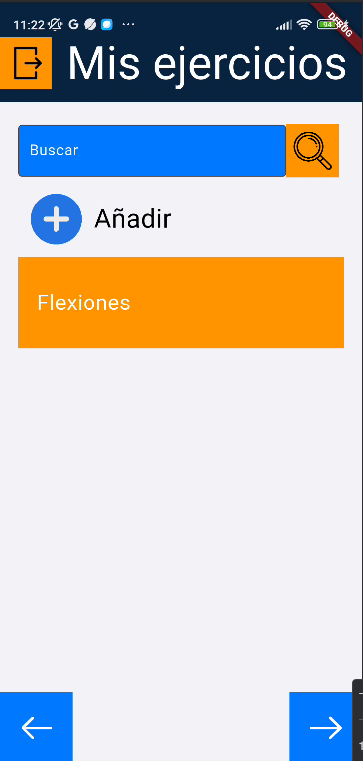
\includegraphics[width=\textwidth]{pantallas/listaEjercicios.png}
    \caption{Lista ejercicios}
    \label{fig:ListaEjer}
\end{figure}

Una de las dificultades de esta funcionalidad fue que esta pantalla debería funcionar como una plantilla, es decir, se han de pasar las funciones de consultas y la clase construiría una lista pasase lo que se pasase, de esta forma se recilclaría mucho código ahorrando tiempo. Lo que se hizo fue una ingeniería inversa, se desarrollo la pantalla forma específica para los ejericios y cuando funcionaba correctamente, se fue abstrayendo el código hasta obtener la clase ListaBusquedaAniadir.

Otro problema encontrado durante las pruebas fue la actualización de la lista, se tuvieron muchos problemas dado que en flutter si se tiene una instancia de un widget llamemoslo A, que forma parte de otro llamado B, si yo llamo a una actualización de la IU desde B porque ha cambiado el contenido se genera una excepción. Como solución, se optó por solo usar la función setState (Usada para actualizar el contenido) dentro del código de la plantilla y cada vez que fuera necesario hacer una actualización desde B recargar otra vez la pantalla entera.

Las pruebas realizadas fueron de caja negra, ir añadiendo elementos para que se hagan visibles en la IU e ir comprobando navegabilidad del menu, el algorítmo de búsqueda y que se actualizaba correctamente al añadir algún objeto.

\HU{
SCRUM-3: Insertar/Borrar/Modificar ejercicio de la lista de ejercicios
}{
	\item Implementar la BD local
	\item Implementar las funciones para las consultas
	\item Implementar las funciones para las modificaciones
	\item Implementar las funciones para el borrado
	\item Implementar boceto de la IU \cref{fig:Datos ejercicio}, para borrar/modificar desde ahí
}{
	\item si se borra un ejercicio, no sale en la lista
	\item si se modifica, sale con los datos modificados
	\item si se inserta, sale en la lista el ejercicio
	\item se enseñan los datos del ejercicio de forma correcta
}

\begin{figure}[H]
   \centering
    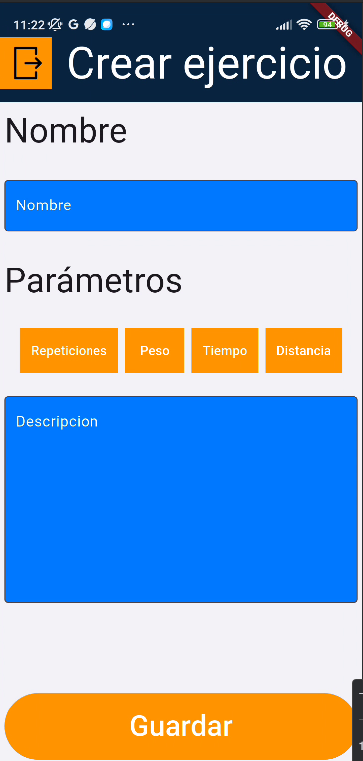
\includegraphics[width=0.8\textwidth]{pantallas/CrearEjercicio.png}
    \caption{Crear ejercicios}
    \label{fig:CrearEjers}
\end{figure}

\begin{figure}[H]
   \centering
    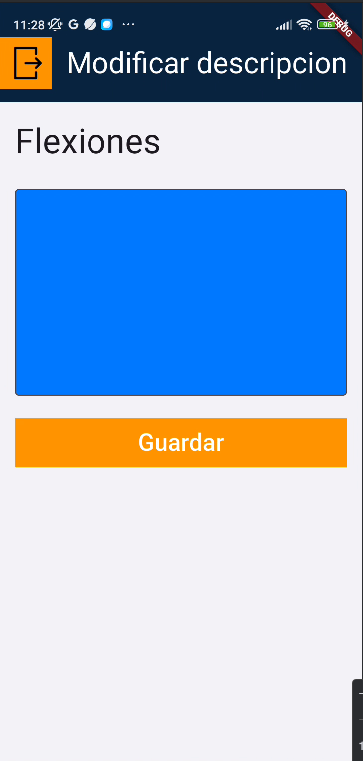
\includegraphics[width=0.8\textwidth]{pantallas/ModDescpEjer.png}
    \caption{Modificar descripcion ejercicios}
    \label{fig:ModDescpEjer}
\end{figure}

Las pruebas realizadas para la SCRUM-3, fueron de caja negra, ir haciendo inserciones y borrados en la BD local para despues hacer consultas y comprobar si los resultados eran correctos. También se comprobó su correcto funcionamiento con el SCRUM-3, corroborando la correcta actualización de los contenidos.

\HU{
SCRUM-43: Añadir meta por parámetro
}{
	\item Implementar la BD local
	\item Implementar las funciones para modificar metas
}{
	\item si existe una meta determinada para ese ejercicio y se quiere insertar una, sustituir la actual
}

\begin{figure}[H]
   \centering
    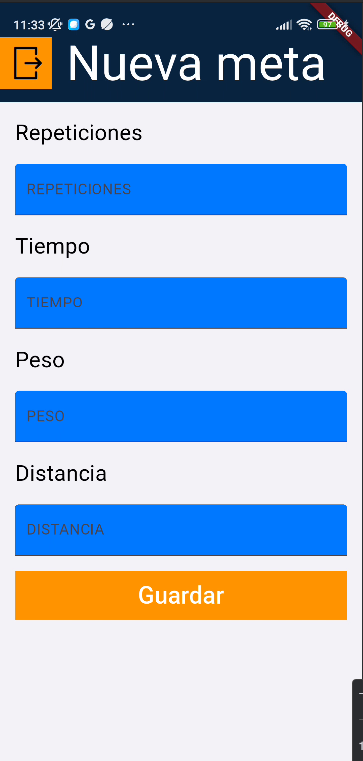
\includegraphics[width=0.8\textwidth]{pantallas/NuevaMeta.png}
    \caption{Nueva meta}
    \label{fig:NuevaMeta}
\end{figure}

El problema de esta iteración fue el como distinguir internamente, si un usuario quiere superar con un valor mayor o menor su meta, es decir, si un usuario quiere aumentar el peso con el que hace un ejercicio o disminuirlo. Al final optó por que solo se pueda aumentar.

Las pruebas realizadas se basaron en añadir valores nuevos de metas tanto erroneos como válidos, para ver como se comportaban las soluciones implementadas a las erratas que pueda introducir el usuario.

\HU{
	SCRUM-29: Pop up de confirmación  
}{
	\item Implementar la confirmación para que pueda ser usado en pantallas distintas
	\item Implementar boceto de IU \cref{fig:Pop up de confirmacion} 
}{
	\item si se ha seleccionado una opcion, se devuelve la opcion seleccionada
}

\begin{figure}[H]
   \centering
    \includegraphics[width=0.8\textwidth]{pantallas/PopUpConfirmacion.png}
    \caption{PopUp Confirmacion}
    \label{fig:PopUpConfirmacion}
\end{figure}

\subsubsection{Estado de la BD local}

Cabe aclarar que la BD local es la memoria persistente de la app que solo existe en el dispositivo que esta instalada la app, se le llama BD local porque tiene una estrucura tipo SQL.

Al finalizar esta iteración, el estado de la BD queda tal y como se muestra en la figura \cref{fig:BD local iteracion 1}
\begin{figure}[H]
   \centering
    \includegraphics[width=\textwidth]{fotos/BDL iteracion 1.png}
    \caption{BD local iteracion 1}
    \label{fig:BD local iteracion 1}
\end{figure}

\subsubsection{Sprint Review 1}
Las primeras iteraciones tienden a ser más lentas debido a la fase inicial del desarrollo. No se completó la totalidad del sprint; quedó pendiente la subtarea de modificar ejercicio en la base de datos(SCRUM-3: Insertar/Borrar/Modificar ejercicio de la lista de ejercicios). Aun así, las expectativas son positivas, ya que se espera un aumento en la velocidad de desarrollo.

La pantalla en la que se enseñan los datos de un ejercicio se modificó para facilitar su lectura y entendimiento, dado que su anterior diseño era confuso.

Otra parte a modificar es la del pop up de confirmación, ya que debido a la poca accesibilidad de los pop ups se sustituirá por una pantalla independiente.

\begin{figure}[h!]
  \centering
  \begin{minipage}[b]{0.45\textwidth}
    \centering
    \includegraphics[width=\textwidth]{fotos/ejerciciosNueva.png}
    \caption{Pantalla nueva}
    \label{fig:pantalla_nueva}
  \end{minipage}
  \hfill
  \begin{minipage}[b]{0.45\textwidth}
    \centering
    \includegraphics[width=\textwidth]{fotos/ejerciciosVieja.png}
    \caption{Pantalla antigua}
    \label{fig:pantalla_vieja}
  \end{minipage}
  \caption{Comparación entre la pantalla nueva y la anterior}
  \label{fig:comparacion_pantallas}
\end{figure}

\subsection{Iteración 2}
Esta iteración se centró en el desarrollo del sistema de sesiones, la API de la aplicación, el backend básico del servidor y la sección de rutinas. Las historias que incluye son las siguientes:

\begin{itemize}
  \item SCRUM-21 Crear/Borrar mi usuario
  \item SCRUM-23 Iniciar/Cerrar sesión
  \item SCRUM-6 Insertar/Borrar/Modificar rutina
  \item SCRUM-4 Buscar rutina en la lista del usuario
  \item SCRUM-31 Crear IU de la lista de las rutinas ELIMINAR
  \item SCRUM-32 Crear IU de pantalla inicial ELIMINAR
  \item SCRUM-33 Implementar menú principal
  \item SCRUM-34 Crear IU datos rutinas ELIMINAR
  \item SCRUM-35 IU lista ejercicios de rutina modificable ELIMINAR
  \item SCRUM-36 Crear IU para crear rutina ELIMINAR
\end{itemize}

También se terminará la historia no finalizada de la iteración anterior(SCRUM-3: Insertar/Borrar/Modificar ejercicio de la lista de ejercicios).

\HU{
SCRUM-33 Implementar menú principal
}{
	\item Implementar el boceto IU \cref{fig:Menu principal}
	\item Añadir accesos a las funcionalidades actuales
}{
	\item si la funcionalidad seleccionada no está implementada, no hacer nada
	\item si la funcionalidad seleccionada está implementada, desplegar ventana de dicha funcionañidad
}

\begin{figure}[H]
   \centering
    \includegraphics[width=0.8\textwidth]{pantallas/MenuPrincipalSemi.png}
    \caption{Menu Principal semifuncional}
    \label{fig:MenuPrincipalSemi}
\end{figure}

Las funcionalidades que no esten disponibles al ser pulsadas no hacen nada.

\HU{
SCRUM-21 Crear/Borrar mi usuario
}{
	\item Implementar bocetos de IU \cref{fig:Crear cuenta 1} ,\cref{fig:Crear cuenta 2}, \cref{fig:Pagina inicial} y la parte necesaria de \cref{fig:Opciones de perfil usuario}
	\item Implementar funciones de inserccion y borrado en el backend
}{
	\item si el usuario que se quiere crear ya existe, informar y pedir que se rellenen los credenciales otra vez
	\item si el usuario que se quiere crear no existe, crear usuario y pasar a la siguiente pantalla
	\item si cualquier dato requerido está en un formato incorrecto ,informar al usuario para que vuelva a rellenar estos
	\item si todos los datos están en el formato correcto ,seguir con la creación del usuario
	\item si se ha creado exitosamente el usuario, volver a la pantalla inicial
	\item si se borra el usuario, borrar el token en el dispositvo y sus credenciales en el backend
}

\begin{figure}[H]
   \centering
    \includegraphics[width=0.8\textwidth]{pantallas/LogSingIn.png}
    \caption{Log In / Sing In}
    \label{fig:LogSingIn}
\end{figure}

\begin{figure}[H]
   \centering
    \includegraphics[width=0.8\textwidth]{pantallas/SingIn1.png}
    \caption{Sing In pantalla 1}
    \label{fig:SingIn1}
\end{figure}

\begin{figure}[H]
   \centering
    \includegraphics[width=0.8\textwidth]{pantallas/SingIn2.png}
    \caption{Sing In pantalla 2}
    \label{fig:SingIn2}
\end{figure}

Las pruebas se realizaron en el backend, la correcta inserción y borrado de usuarios. Cuando se crea correctamente un usuario se redirige a la pantalla inicial. Si se intenta crear un usuario ya existente, se lanza un aviso.

\HU{
SCRUM-23 Iniciar/Cerrar sesión
}{
	\item Implementar el boceto IU \cref{fig:Inicio de sesion} y parte necesaria de \cref{fig:Opciones de perfil usuario}
	\item Implementar función de consulta en el backend
}{
	\item si el usuario con esa contraseña no existe, informar al usuario
	\item si el usuario con esa contraseña existe, devolver un token para su guardado y guardar usuario 
	\item si el usuario quiere cerrar sesión, borrar token y nombre del usuario del dispositivo y volver a la pantalla inicial \cref{fig:Pagina inicial}
}

\begin{figure}[H]
   \centering
    \includegraphics[width=0.8\textwidth]{pantallas/LogIn.png}
    \caption{Log In}
    \label{fig:LogIn}
\end{figure}

\begin{figure}[H]
   \centering
    \includegraphics[width=0.8\textwidth]{pantallas/OpcUser.png}
    \caption{Opciones Usuario}
    \label{fig:Opciones Usuario}
\end{figure}

Al hacer el login correctamente se otorga un token que no hay que renovar hasta el día siguiente, al cerrar sesión se borra automaticamente. Las pruebas realizadas se basaron en comprobar el correcto alamacenaje y borrado del token, usando la librería de secure storage de flutter, que nos permite guardar variables de forma permanente y encriptada con un facil acceso, como si fuera un map.

Para comprobar la veracidad de los credenciales se implementó la parte básica del backend, un server con una BD(mySQL) que guardará los usuarios con sus contraseñas y la parte implementada usando Express.js(Node.js) para escuchar peticiones, el server también será el encargado de proporcionar y verificar los tokens. La comunicación entre servidor y cliente (el dispositivo en el que esta instalada la app) se usan peticiones HTTP, en futuro se puede migrar a HTTPS si es necesaria mas seguridad.

\HU{
SCRUM-4 Buscar rutina en la lista del usuario
}{
	\item Implementar IU del boceto \cref{fig:Lista rutinas}
	\item Implementar lo necesario en la BD local
	\item Implementar algorítmo de búsqueda
	\item Implementar acceso a la rutina seleccionada
}{
	\item si no existe la rutina buscada, no enseñar acceso en pantalla
	\item si existe la rutina buscada, enseñar acceso en pantalla
}

\begin{figure}[H]
   \centering
    \includegraphics[width=0.8\textwidth]{pantallas/listaRutinas.png}
    \caption{Lista Rutinas}
    \label{fig:listaRutinas}
\end{figure}

Esta funcionalidad se abarcó aprovechando lo implementado en la iteración anterior del SCRUM-26. Se realizaron las mismas pruebas pero relacionadas con las rutinas.

\HU{
SCRUM-6 Insertar/Borrar/Modificar rutina
}{
	\item Implementar las insercciones en para la BD local
	\item Implementar los borrados para la BD local
	\item Implementar las modificaciones para la BD local
}{
	\item si se hace una insercción, que el elemento insertado sea visible en la lista de ejercicios
	\item si se hace un borrado, que el elemento desaparezca de la lista
	\item si se hace una modificación, que se hagan visibles los cambios al momento
	\item si hay algún fallo en alguna de estas operaciones, informar al usuario con el motivo
}

\begin{figure}[H]
   \centering
    \includegraphics[width=0.8\textwidth]{pantallas/DatosRutina.png}
    \caption{Datos Rutina}
    \label{fig:DatosRutina}
\end{figure}

\begin{figure}[H]
   \centering
    \includegraphics[width=0.8\textwidth]{pantallas/crearRutina.png}
    \caption{Crear Rutina}
    \label{fig:crearRutina}
\end{figure}

\begin{figure}[H]
   \centering
    \includegraphics[width=0.8\textwidth]{pantallas/listaEjerRutina.png}
    \caption{Lista Ejercicios Rutina}
    \label{fig:listaEjerRutina}
\end{figure}

\begin{figure}[H]
   \centering
    \includegraphics[width=0.8\textwidth]{pantallas/modRutina.png}
    \caption{Modificar Rutina}
    \label{fig:modRutina}
\end{figure}

\begin{figure}[H]
   \centering
    \includegraphics[width=0.8\textwidth]{pantallas/listaAddEjerRut.png}
    \caption{Lista añadir ejercicio a rutina}
    \label{fig:listaAddEjerRut}
\end{figure}

Como se puede observar se rescato mucho código de la primera iteración, solo hubo que hacer unas pequeñas modificaciones en la clase plantilla usada para crear las pantallas \cref{fig:listaEjerRutina} y \cref{fig:listaAddEjerRut}, en concreto a la pantalla de la lista de ejercicios preteneciente a la rutina se le realizaron pruebas para ver la correcta actualización de los contenidos.

En la pantalla \cref{fig:modRutina} la unica prueba realizada fue comprobar la correcta modifición en la BD local y su correcta visualización en la misma.

La funcionalidad de compartir todavía no está implementada.

\subsubsection{Sprint Review 2}
Se sugirieron mejoras menores como el ajuste de tamaños e iconos en los botones de la sección de creación de rutinas.

También se modificó la funcionalidad de compartir rutinas. Ahora todas son modificables, eliminando la distinción entre rutinas descargadas (antes no modificables) y creadas (modificables). Esto mejora la experiencia del usuario: si desea volver a una rutina original, simplemente la puede volver a buscar y descargar.

Se cumplieron todas las funcionalidades en este sprint.

\subsubsection{Estado de la BD local}

\begin{figure}[H]
   \centering
    \includegraphics[width=\textwidth]{fotos/BDL iteracion 2.png}
    \caption{BD local iteracion 2}
    \label{fig:BD local iteracion 2}
\end{figure}

Se añadieron las tablas de ejercicios y marcas, una o varias marcas siempre están relacionadas con un ejercicio, de esta forma, se saben todas las marcas de un ejercicio y si se elimina un ejercicio sus marcas también desaparecen.

\subsubsection{Estado de la BD backend} 

Antes de seguir, la BD del backend es donde se guardan los usuarios registrados y sus rutinas compartidas. Para diferenciarlo de la BD local, que es el almacenamiento interno del dispositivo.

\begin{figure}[H]
   \centering
    \includegraphics[width=0.7\textwidth]{fotos/BD be iteracion 2.png}
    \caption{BD backend iteracion 2}
    \label{fig:BD backend iteracion 2}
\end{figure}

\subsection{Iteración 3}
Esta iteración se centró en desarrollar la funcionalidad para compartir rutinas entre usuarios, incluyendo la subida, visualización y descarga de rutinas. Además, se comenzó a implementar la funcionalidad de resumen de datos para optimizar el uso de la memoria local. Incluye las siguientes historias:

\begin{itemize}
  \item SCRUM-2 Establecer peso objetivo
  \item SCRUM-37 Crear IU del perfil del usuario ELIMINAR
  \item SCRUM-42 Copiar rutina
  \item SCRUM-10 Enseñar datos de una rutina a descargar
  \item SCRUM-11 Compartir mi rutina
  \item SCRUM-39 Buscar rutinas para descargar
  \item SCRUM-9 Revisar datos para ver si el descanso es necesario
  \item SCRUM-22 Resumir datos
  \item SCRUM-40 IU del pop up de resumir datos ELIMINAR
  \item SCRUM-41 IU desplegable rutina ELIMINAR
\end{itemize}
\HU{
SCRUM-2 Establecer peso objetivo
}{
	\item Implementar la parte necesaria de \cref{fig:Opciones de perfil usuario}
	\item Implementar el almacenaje de ese peso objetivo
}{
	\item si el peso objetivo está en el formato correcto, guardar
	\item si el peso objetivo no está en el formato correcto, enseñar una alerta para su corrección
}


\begin{figure}[H]
   \centering
    \includegraphics[width=0.8\textwidth]{pantallas/pesoObj.png}
    \caption{Peso Objetivo}
    \label{fig:pesoObj}
\end{figure}

Para guardar el peso, en esta iteración como no se crearan las tablas para guardas los pesajes del usuario se guardará usando secure storage, es una solución temporal. En para esta funcionalidad se hicieron pruebas para comprobar la correcta insercción del formato del peso, que no se añadan letras. que se admitan comas y puntos, que solo se use un decimal.

\HU{
SCRUM-11 Compartir mi rutina
}{
	\item Implementar la BD en el backend
	\item Implementar funciones de inserción en la API
}{
	\item si la rutina no contiene ejercicios, no permitir su subida al servidor
	\item si la rutina contiene ejercicios, permitir la subida al servidor
}

Esta funcionalidad dió muchos quebraderos de cabeza ya que varios usuarios podrían tener una rutina con el mismo nombre y al mismo tiempo al descargar una rutina, un usuario podría tener un ejercicio llamado igual o varios usuario podrían tener en la nube varios ejercicios subidos con el mismo nombre. Esto son solo uno de los pocos problemas encontrados en esta funcionalidad.

Para solucionar algunos de estos problemas se hizo lo siguiente, en el backend en la BD los ejercicios y rutinas serán guardados usando como clave primaria un id que sera un int autoincrementado, evitando problemas integridad. Tambíén cuando sean referenciados en la BD se hará usando su id.

\begin{figure}[H]
   \centering
    \includegraphics[width=0.8\textwidth]{pantallas/rutinaMiaOComp.png}
    \caption{Elegir lista compartida por el usuario o locales}
    \label{fig:rutinaMiaOComp}
\end{figure}

\begin{figure}[H]
   \centering
    \includegraphics[width=0.8\textwidth]{pantallas/rutinasCompUsuario.png}
    \caption{Rutinas compartidas por el usuario}
    \label{fig:rutinasCompUsuario}
\end{figure}

\begin{figure}[H]
   \centering
    \includegraphics[width=0.8\textwidth]{pantallas/DatosMiRutinaComp.png}
    \caption{Datos rutinas compartidas por el usuario}
    \label{fig:DatosMiRutinaComp}
\end{figure}

\HU{
SCRUM-39 Buscar rutinas para descargar
}{
	\item Implementar funciones de consultas en la API
	\item Implementar IU de busqueda de rutinas por usuario creador y por nombre de rutina
}{
	\item si busco un usuario que no existe, no se muestra ningún acceso en la IU
	\item si busco un usuario existente, se muestra su acceso en la IU
	\item si busco una rutina que no existe, no se muestra ningún acceso en la IU
	\item si busco una rutina existente, se muestra su acceso en la IU
}

Se puede buscar tanto un usuario y ver las rutinas que ha subido o directamente buscar por nombre de la rutina. Se recicló la pantalla de lista de rutinas \cref{fig:Lista rutinas}, y se implementó la pantalla de DatosRutinaComp, que se usa para ver datos de pantallas compartidas. También para hacer más fácil la distinción entre rutinas del propio usuario y las que ha compartido se añadió otra pantalla exclusivamente de pantallas compartidas, en la cual se nos permite elminar de la nube las rutinas elegidas.

Para solucionar los problemas de integridad generados en el dispositivo del usuario, al descargar una rutina se le añadirá a su nombre y al de los ejercicios que contiene el nombre del creador, y si aún así hay problemas de integridad, se añade al nombre de la rutina y/o ejercicio el número de copia que es dentro del dispositivo. Desarrollando lo anterior, al descargar una rutina llamada "Flexiones" del usuario "Paco", en el dispositivo que realiza la descarga se llamará "Flexiones-Paco", si en el dispisitivo en el que se realiza la descarga ya existe otra rutina llamada "Flexiones-Paco", la descargada se llamará en el dispositivo "Flexiones-Paco(1)".La integridad de los ejercicios se trata igual.

\begin{figure}[H]
   \centering
    \includegraphics[width=0.8\textwidth]{pantallas/buscarRutinasNomOUser.png}
    \caption{Buscar rutinas o usuario}
    \label{fig:buscarRutinasNomOUser}
\end{figure}

\begin{figure}[H]
   \centering
    \includegraphics[width=0.8\textwidth]{pantallas/buscarRutina.png}
    \caption{Buscar rutinas por su nombre}
    \label{fig:buscarRutina}
\end{figure}

\begin{figure}[H]
   \centering
    \includegraphics[width=0.8\textwidth]{pantallas/buscarUser.png}
    \caption{Buscar usuarios}
    \label{fig:buscarUser}
\end{figure}

\HU{
SCRUM-10 Enseñar datos de una rutina a descargar
}{
	\item Implementar el IU pop up
	\item Implementar las funciones de consulta en la API
	\item Implementar las funciones de inserción en la BD local
}{
	\item si se va a descargar la rutina y el usuario tiene en el dispositivo otra con el mismo nombre, un algorítmo resolverá este problema
	\item si se va a descargar la rutina y el usuario no tiene en el dispositivo otra con el mismo nombre, descargar normalmente
}

Es la misma pantalla para ver nuestras rutinas subidas, reciclamos código, la única diferencia es que no podedmos elminarla de la nube, solo podemos descargarla.

\begin{figure}[H]
   \centering
    \includegraphics[width=0.8\textwidth]{pantallas/datosRutinasDesc.png}
    \caption{Datos rutinas para descargar}
    \label{fig:datosRutinasDesc}
\end{figure}

\HU{
SCRUM-42 Copiar rutina
}{
	\item Añadir al boceto IU de datos rutina \cref{fig:Datos rutina modificable} esta funcionalidad
	\item Implementar la IU resultante de la tarea anterior
	\item Implementar las consultas e inserciones necesarias en la BD local
}{
	\item si hay algún problema por coincidencia de nombres, un algorítmo resolverá este problema
	\item si no hay algún problema por coincidencia de nombres, copiar
}

\subsubsection{Funcionalidad descartada}

Durante la realización de estas tareas de usuario, se dió notoriedad a que las historias restantes de este sprint (SCRUM-9 Revisar datos para ver si el descanso es necesario y SCRUM-22 Resumir datos) no pueden ser implementadas en este punto del desarrollo. Se pospondrán para su futura implementación.

Se ha decidido dar menos prioridad y que por tanto no se abordará en este TFG por limitaciones de tiempo en concreto el SCRUM-9 (Revisar datos para ver si el descanso es necesario), porque necesitaría los datos de un smartwatch y ha sido una funcionalidad previamente descartada.

También se ha reducido la prioridad de SCRUM-42 (Copiar rutina), dado que aporta poco valor a la app.

Se decidió adelantar otras, pero debido a los problemas encontrados durante esta iteración no se pudieron realizar.

\subsubsection{Estado BD local}

No ha habido cambios respecto a la iteración anterior

\subsubsection{Estado BD backend}

\begin{figure}[H]
   \centering
    \includegraphics[width=\textwidth]{fotos/BD be iteracion 3.png}
    \caption{BD backend iteracion 3}
    \label{fig:BD be iteracion 3}
\end{figure}

\subsubsection{Sprint Review 3}

Se identificaron dos errores principales de planificación:

\begin{description}
  \item[Error 1:] Se planificó implementar la funcionalidad de resumir datos sin haber completado la obtención de datos. \\ \textbf{Solución:} Replanificar los sprints.
\end{description}

Los imprevistos y problemas surgidos durante el desarrollo han permitido detectar \textit{bugs}, errores de dise\~no y carencias funcionales que de otro modo podrían haber pasado desapercibidos. Gracias a ello, se han podido proponer nuevas funcionalidades y mejorar las ya existentes, lo cual contribuye significativamente a aumentar la calidad global de la aplicación.

Algunas funcionalidades propuestas como mejora son:

\begin{itemize}
  \item Verificar el token del usuario antes de permitir la subida de rutinas, para evitar suplantación.
  \item Al seleccionar la opción de borrar usuario del dispositivo, eliminar también la base de datos local asociada.
  \item Crear una base de datos local independiente para cada nuevo usuario creado en un dispositivo.
  \item Posibilidad de editar el nombre de una rutina.
  \item Marcar los ejercicios eliminados con una \textit{flag}, para evitar que se inicien rutinas que los contengan.
  \item Marcar a los usuarios permanentemente eliminados con una \textit{flag}, para proceder a eliminarlos en los dispositvos.
\end{itemize}

Estas funcionalidades están pensadas para aportar mayor \textbf{seguridad}, \textbf{integridad} y \textbf{calidad} al producto final.

En esta review se estuvo debatiendo si quitar las funcionalidades relacionadas con el smartwatch, por cuestiones de tiempo, ya que con las funcionalidades añadidas en el capitulo anterior se va ajustando el plazo.

En esta iteración se tenía pensado implementar la funcionalidad de resumir los datos, no obstante, al no tener implementada la parte en la que guardo las marcas de los entrenamientos, no puedo trabajar en esa funcionalidad. Por lo tanto, se ha pospuesto para la próxima iteración. También se le dió el visto bueno a la implementación de las funcionalidades previamente expuestas durante el desarrollo.

\subsection{Iteración 4}

En esta iteración se tiene pensado implementar la funcionalidad del calendario, donde el usuario podrá ver su planificación y acceder a sus marcas. Por otro lado, también se implementarán las funcionalidades nuevas del sprint anterior y las nuevas pantallas.

\begin{itemize}
	  \item SCRUM-39 Detectar metas cumplidas en los ejercicios despues del entrenamiento
	  \item SCRUM-1 Registrar peso por día
	  \item SCRUM-19 Realizar el flujo del entrenamiento
	  \item SCRUM-44: Implementar calendario
\end{itemize}

\HU{
SCRUM-44: Implementar calendario
}{
	\item Implementar la IU e insertarla en el menu principal \cref{fig:Menu principal}
	\item Implementar en la BD local
	\item Implementar funciones de inserción en BD local
	\item Implementar funciones de consulta en BD local
	\item Implementar funciones de borrado en BD local
	\item Implementar un acceso para ver los datos registrados sobre un día en concreto
}{
	\item si un día no tiene una rutina asignada, se considera descanso
	\item si un día tiene una rutina asignada, no hay marcas registradas y el día ya ha pasado, no se enseñará información, ya que se considera no entrenado
	\item si un día tiene una rutina asignada, no hay marcas registradas pero es hoy, se enseñará un acceso para empezar el entrenamiento, se considera que el usuario todavía no ha entrenado
	\item si un día tiene una rutina asignada, pero es futuro, no se enseñará un acceso para empezar el entrenamiento
	\item si un día tiene una rutina asignada y hay marcas registradas sea el día actual o pasado, se mostrará información de las marcas, sin acceso a entrenamiento
}
\HU{
SCRUM-19 Realizar el flujo del entrenamiento
}{
	\item Implementar IU de las pantallas de entrenamientos(de la \cref{fig:Lista ejercicios del entrenamiento actual}  a la \cref{fig:Fin entrenamiento})
	\item Implementar una clase que controle el cambio entre distintas pantallas y el guardado de marcas
}{
	\item si la rutina asignada para un día, no tiene ejercicios y se desea iniciar el entrenamiento, se muestra por pantalla una alerta y no se permite continuar con el entrenamiento
	\item si la rutina asignada para un día, tiene ejercicios, comienza el recorrido entre IUs
	\item si es la primera serie de un ejercicio, no se permite terminar el ejercicio
	\item si no es la primera serie de un ejercicio, se permite terminar el ejercicio
	\item si acaba una serie, no se permitirá acabar el ejercicio o continuar con este hasta que termine el tiempo de descanso que se muestra en pantalla
	\item si finaliza el último ejercicio de la lista, fin del entrenamiento, se devuelve al usuario al menú principal
}
\HU{
SCRUM-39 Detectar metas cumplidas en los ejercicios despues del entrenamiento
}{
	\item Implementar bocetos de IU \cref{fig:Metas cumplidas}
	\item Implementar lógica para comparar marcas y metas despues de acabar el entrenamiento en la clase que controla el flujo del entrenamiento
}{
	\item si en un ejercicio no se ha cumplido la meta, no se enseña nada
	\item si en un ejercicio cumplimos una meta, se enseña en que ejercicio se cumplió la meta
}
\HU{
SCRUM-1 Registrar peso por día
}{
	\item Implementar boceto de IU \cref{fig:Datos detallados entrenamiento terminado}
	\item Implementar en BD local
	\item Implementar funciones de inserción
	\item Implementar funciones de consulta
	\item Implementar lógica para determinar si un usuario quiere subir o bajar de peso
}{
	\item si se introduce algún dato como formato incorrecto, se muestra una alerta por pantalla
	\item si se introducen los datos en formato correcto, se guarda
}

En esta iteración hay pocas funcionalidades comparadas con otras, porque el flujo del entrenamiento es una funcionalidad muy grande. A parte se añade esta funcionalidad que también se va a realizar en esta iteración, SCRUM-44 Implementar calendario.

\subsubsection{Paquete tableCalendar} % al igual que en iteraciones previas, asocia esto a la historia concreta afectada y a sus resultados.

Es un paquete de flutter, que permite implementar y customizar un calendario, de forma fácil y rápida. También permite trabajar con información para reflejarla en las fechass del calendario.

\begin{figure}[h!]
    \centering
    \includegraphics[width=0.45\textwidth]{fotos/PantallaCalendario.png}
    \caption{Pantalla Calendario}
    \label{fig:Pantalla Calendario}
\end{figure}

Existen varios formatos de calendario preimplementados, que cambian el numero de dias en pantalla, se escogió este porque es el que menos problemas da en pantalla y más cómodo para las interacciones que busca el usuario.

\subsubsection{Pantallas cambiadas por pop ups}

La solución que se ha dado para que este problema no quite mucho tiempo de desarrollo es la siguiente, reciclar todo el contenido posible del interior de los pop ups y plasmarlo tal cual en una pantalla. Dado que los diseños implementados eran buenos, quitando algún fallo que puedan dar por este cambio de formato.

Los pop ups que se cambiaron son los siguientes:

\begin{itemize}
	\item Los pop ups de confirmacion
	\item Crear ejercicios
	\item Modificar ejercicios
	\item Nueva meta en un ejercicio
	\item Crear rutinas
	\item Modificar rutinas
	\item Modificar ejercicios de una rutina
	\item Información de una rutina a descargar
	\item Modificar informacion del perfil del usuario
\end{itemize}

Por consecuencia las futuras funcionalidades en la que se mencionan los pop ups, pasaran a ser pantallas completas.

\subsubsection{Cambios en el backend}

Los cambios en el backend están relacionados con las siguientes funcionalidades propuestas en la iteracion anterior:

\begin{itemize}
	\item Cambio 1: Verificar el token del usuario antes de permitir la subida de rutinas, para evitar suplantación.
  	\item Cambio 2: Marcar a los usuarios permanentemente eliminados con una \textit{flag}, para proceder a eliminarlos en los dispositvos.
\end{itemize}

Cambio 1: la solución implementada es la siguiente, a todas las funciones que puedan ser potencialmente victimas de una suplantación(via peticion normal de http), se les ha añadido un middleware, una función que se ejecuta antes para verificar el token. Express.js permite implementar esto rapidamente

Cambio 2: de primeras se pensó en usar una flag, pero finalmente para evitar perdida de rendimiento al momento de que el usuario realize un entrenamiento(que es cuando en un principio se tenía pensado borrar el ejercicio), se optó por modificar la lista de ejercicios de la rutina al momento de borrar el ejercicio. El número de consultas iba a ser el mismo, pero se ahorra memoria, ya que no añadimos una columna más a la tabla de ejercicios

\subsubsection{Flujo entrenamiento}

Para acaparar esta funcionalidad, se ha implementado una clase aparte encargada del desarrollo de esta parte de la app. Se ha decidido así ya que es una lógica más compleja y es conveniente tenerla separada de la IU.

Esta clase, solo se puede crear de forma util llamando a un método estático de la propia clase (se hace así ya que necesita hacer operaciones asíncronas para obtener los datos necesarios), este método estático me devuelve la instancia con la que voy a trabajar. Se llama al método ejecutar de la instancia creada y sola se encarga de mostrar las pantallas al usuario, guardar los datos y de comparar las metas que se propuso el usuario.

Aquí un diagrama de actividades que explica la tarea de esta clase:

\begin{figure}[H]
    \centering
    \includegraphics[width=0.75\textwidth]{tablas/FlujoEntrenamiento.png}
    \caption{Flujo entrenamiento}
    \label{fig:Flujo entrenamiento}
\end{figure}

\subsubsection{Estado de la BD local}

\begin{figure}[H]
    \centering
    \includegraphics[width=\textwidth]{fotos/BDL iteracion 4.png}
    \caption{BD local iteración 4}
    \label{fig:BDL iteracion 4}
\end{figure}

\subsubsection{Estado BD backend}

No sufrió cambios respecto a la iteración anterior

\subsubsection{Sprint review 4}

En esta review se ha propuesto que despues de los entrenamientos se les enseñe a los usuarios las metas que tenían establecidas siempre, aunque no la hayan superado, evitando siempre el feedback negativo al usuario.

\subsection{Iteraci\'on 5} %Falta actualizar esto

Debido a retrasos y problemas durante el desarrollo esta será la última iteración, que se dedicará a la implementación de gráficas para representar los datos requeridos por el usuario. Dado al tiempo limitado que se poseé la implementación de la IA se aplazará al máximo e incluso siendo posible su descarte.
